% !TeX root = ../main.tex

\section{Results}
\subsection{Data set}
\begin{frame}
    \frametitle{Epinions data set}
    \vspace{-2cm}
    \begin{columns}
    \column{0.5\textwidth}
    \begin{table}
        \centering
        \caption{Epinions Sample}
        \small
        \begin{tabular}{ |c|c|c| }
            \hline
            \textbf{user} & \textbf{item} & \textbf{Rating} \\
            \hline
            36153 & 62461 & 5 \\
            \hline
            427 & 38005 & 5  \\
            \hline
            751 & 53361 & 4 \\
            \hline
            11001 & 118950 & 4 \\
            \hline
            1169 & 66176 & 5 \\
            \hline
            9808 & 84459 & 2 \\
            \hline
            85 & 7446 & 4 \\
            \hline
            14717 & 3397 & 2 \\
            \hline
        \end{tabular}
    \end{table}
    \column{0.5\textwidth}
    \begin{table}
        \centering
        \caption{Epinions Descriptive}
        \small
        \begin{tabular}{ |c|c|c|c| }
            \hline
            &\textbf{Ratings Matrix} & \textbf{Train} & \textbf{Test}\\
            \hline
            count & 664824 & 520203 & 144621\\
            \hline
            mean & 3.9917 & 3.99 & 3.9975\\
            \hline
            std & 1.2068 & 1.2072 & 1.2053\\
            \hline
            min & 1 & 1 & 1\\
            \hline
            25\% & 3 & 3 & 3\\
            \hline
            50\% & 4 & 4 & 4\\
            \hline
            75\% & 5 & 5 & 5\\
            \hline
            max & 5 & 5 & 5\\
            \hline
        \end{tabular}
    \end{table}
\end{columns}
\end{frame}
\subsection{Evaluation Metrics}
\begin{frame}[t]
    \vspace{-1cm}
    \hspace{15mm}\underline{\textbf{Single Model}}  \hspace{5cm}\underline{\textbf{Combined Models}}
    \frametitle{Evaluation Metrics}
    \begin{columns}
    \column{0.4\textwidth}
    \begin{flalign*}
            RMSE &= \sqrt{\frac{\sum_{(u,i) \in \mathcal{T}(r_{u,i} - \hat{r}_{u,i})^2}}{n}} \\
            MAE  &= \frac{\sum_{(u,i) \in \mathcal{T}\left|r_{u,i} - \hat{r}_{u,i}\right|}}{n} \\
            RMSUE &= \frac{1}{n}\sum_{u \in \mathcal{T}}\sqrt{\frac{\sum_{i \in \mathcal{I}_u(r_{u,i} - \hat{r}_{u,i})^2}}{n_u}} \\
            MAUE &= \frac{1}{n}\sum_{u \in \mathcal{T}}\frac{\sum_{i \in \mathcal{I}_u\mathopen|r_{u,i} - \hat{r}_{u,i}\mathclose|}}{n_u}\\
    \end{flalign*}
    \vspace{3cm}
    \column{0.6\textwidth}
    \small
    \begin{flalign*}
        RMSE_{Total} &= \sqrt{\frac{n_{KNN}*RMSE_{KNN}^2 + n_{R-KNN}*RMSE_{R-KNN}^2}{n_{KNN} + n_{R-KNN}}}\\
        MAE_{Total} &= \frac{n_{KNN}*MAE_{KNN} + n_{R-KNN}*MAE_{R-KNN}}{n_{KNN} + n_{R-KNN}}
    \end{flalign*}
    \centering
    \footnotesize
    \begin{itemize}
        \item $\mathcal{T}$ is the test set
        \item $r_{u,i}$ is the truth value of a rating for $user_u$ to $item_i$
        \item $\hat{r_{u,i}}$ is the prediction value of a rating for $user_u$ to $item_i$
        \item $n$ is the number of rating predictions
    \end{itemize}
    \vspace{5cm}
    \end{columns}
\end{frame}

\subsection{Results}
\begin{frame}
    \frametitle{Volume of Predictions}
    \vspace{-1.6cm}
    \begin{table}
\centering
\caption{Ratings Predicted with KNN and Recursive-KNN}
\footnotesize
\begin{tabular}{ccc|ccc|c}
\multicolumn{3}{c|}{\textbf{USERS}}            & \multicolumn{3}{c|}{\textbf{ITEMS}}            &                          \\ \cline{1-6}
\textbf{KNN} & \textbf{R-KNN} & \textbf{TOTAL} & \textbf{KNN} & \textbf{R-KNN} & \textbf{TOTAL} & \textbf{SIMILARITY}      \\ \hline
88379        & 34392          & 122771         & 89800        & 33315          & 123115         & Adjusted Cosine          \\
100311       & 24122          & 124433         & 100311       & 24122          & 124433         & Cosine                   \\
100311       & 24122          & 124433         & 100311       & 24122          & 124433         & Jaccard                  \\
93924        & 29747          & 123671         & 94528        & 29203          & 123731         & MAD                      \\
93924        & 29747          & 123671         & 94528        & 29203          & 123731         & MSD                      \\
88379        & 34392          & 122771         & 89800        & 33315          & 123115         & Modified Adjusted Cosine \\
100311       & 24122          & 124433         & 100311       & 24122          & 124433         & Modified Cosine          \\
59017        & 40470          & 99487          & 54644        & 34096          & 88740          & Modified Pearson 1       \\
89936        & 28183          & 118119         & 84511        & 24357          & 108868         & Modified Pearson 2       \\
89936        & 28183          & 118119         & 84511        & 24357          & 108868         & Pearson
\end{tabular}
\end{table}
\end{frame}
\begin{frame}[t]
    \frametitle{User-based KNN and Total RMSE}
    \vspace{-0.7cm}
    \begin{columns}
        \column{0.5\textwidth}
        \centering
        \underline{\textbf{KNN}}
    \begin{figure}
    \centering
    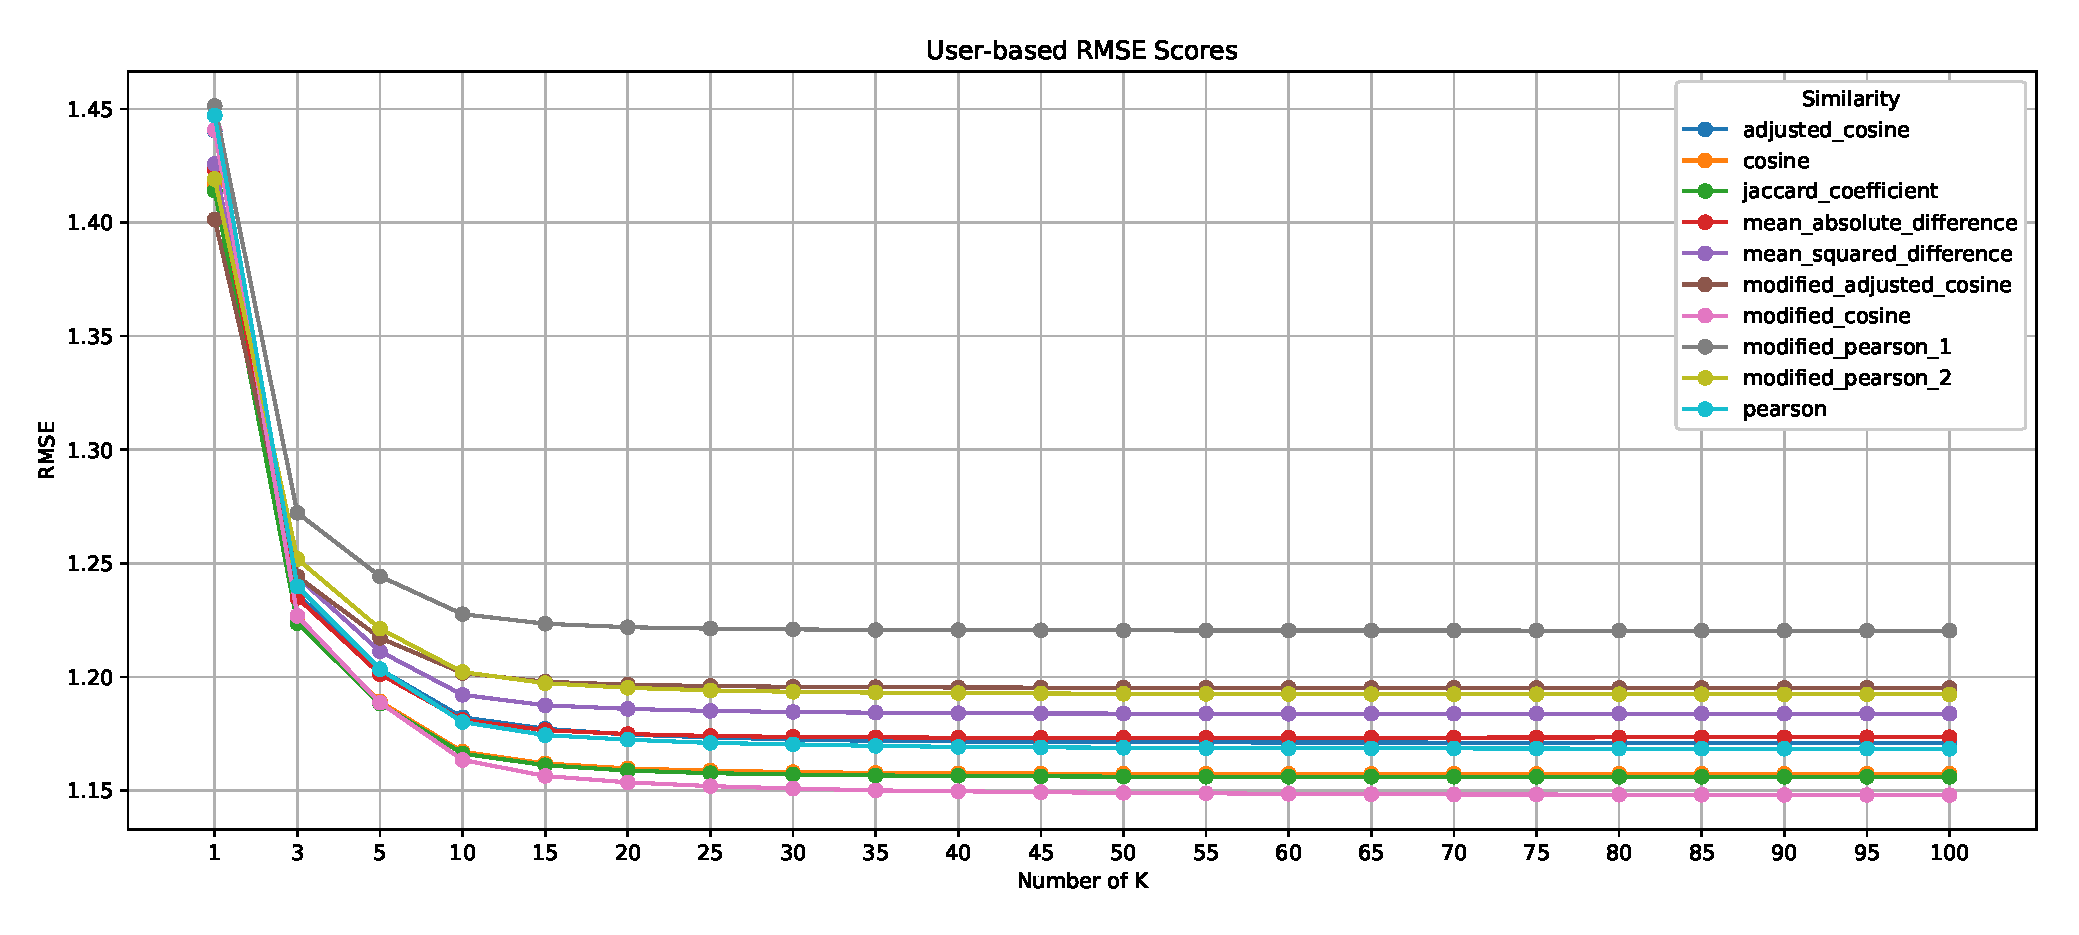
\includegraphics[width=1\textwidth,height=0.6\textheight]{User_RMSE_KNN.eps}
    \end{figure}
    \centering
    \tiny
    Modified cosine at K=100, RMSE=1.1479835373
        \column{0.5\textwidth}
        \centering
        \underline{\textbf{Total}}
    \begin{figure}
    \centering
    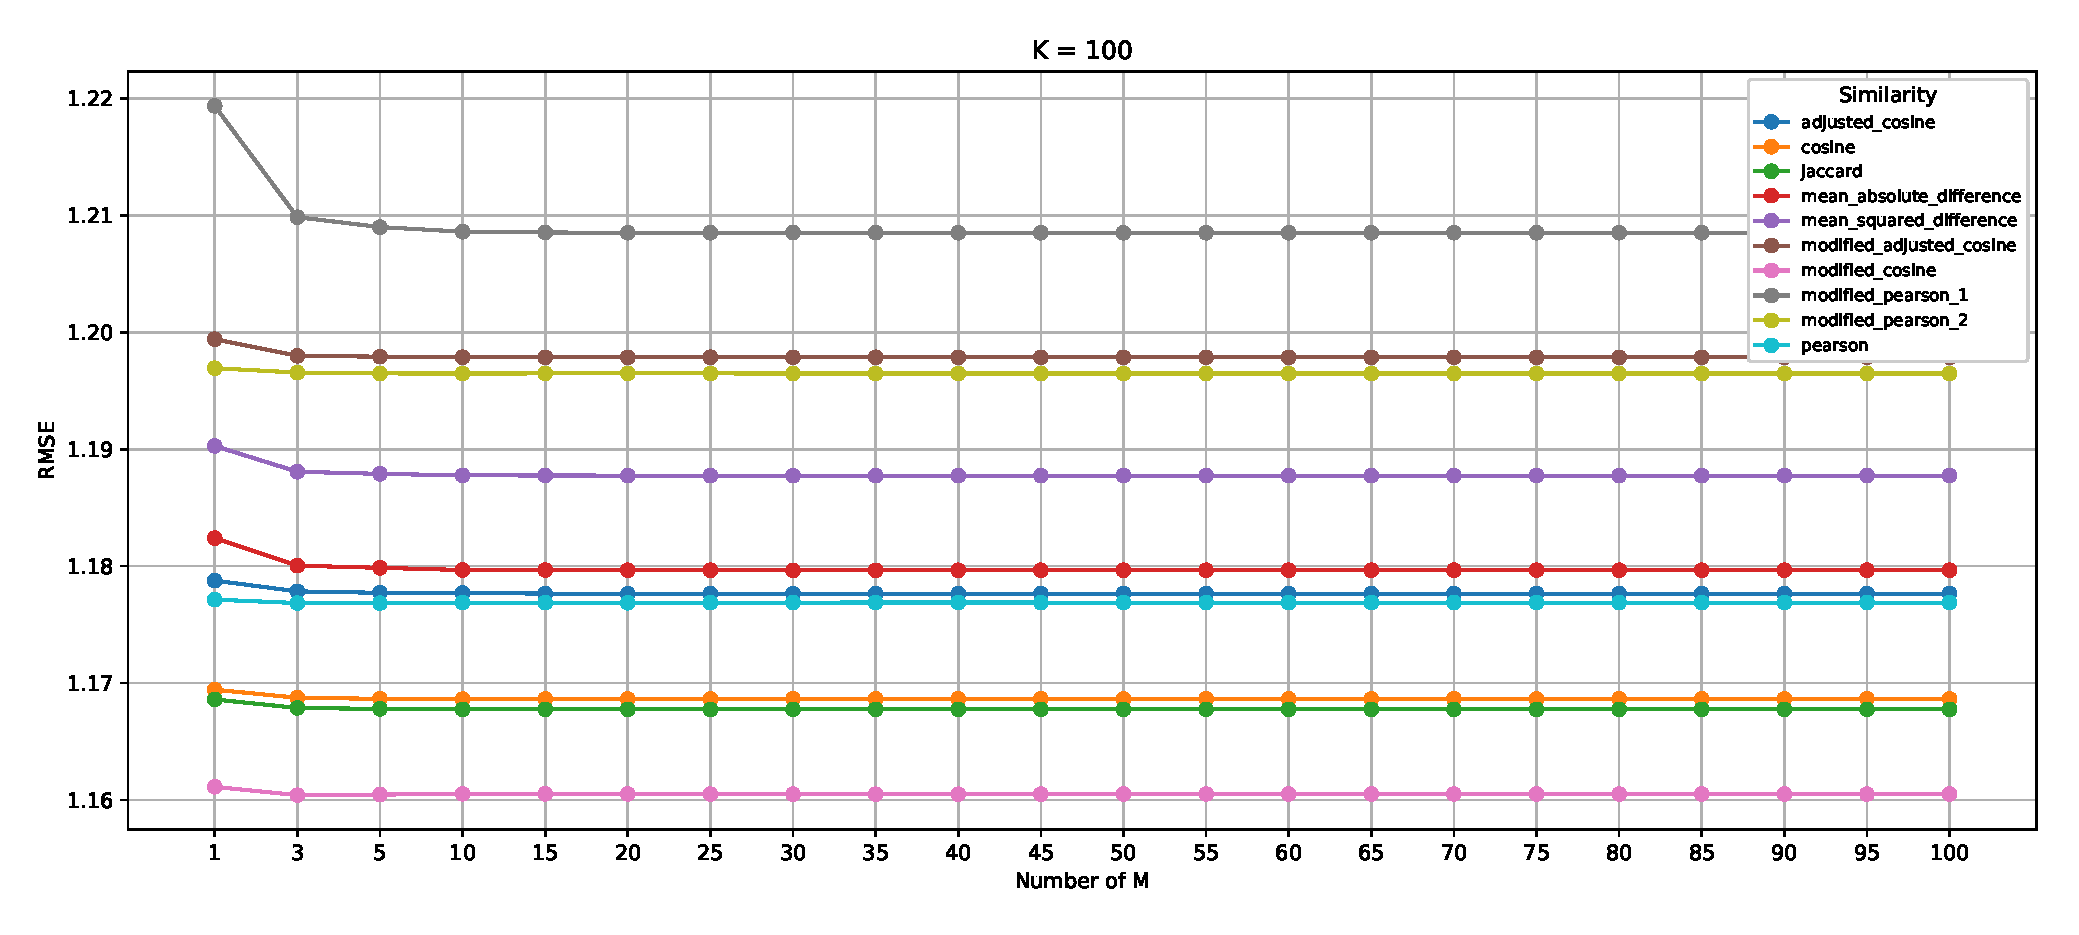
\includegraphics[width=1\textwidth,height=0.6\textheight]{evaluation_user_rmse.eps}
    \end{figure}
    \centering
    \tiny
    Modified cosine at K=100 \& M=3, RMSE=1.1604146071
\end{columns}
\end{frame}
\begin{frame}[t]
    \frametitle{User-based KNN and Total MAE}
        \vspace{-0.7cm}
        \begin{columns}
            \column{0.5\textwidth}
            \centering
            \underline{\textbf{KNN}}
        \begin{figure}
        \centering
        \includegraphics[width=1\textwidth,height=0.6\textheight]{User_MAE_KNN.eps}
        \end{figure}
        \centering
        \tiny
        Jaccard coefficient at K=50, MAE=0.8518433005
            \column{0.5\textwidth}
            \centering
            \underline{\textbf{Total}}
        \begin{figure}
        \centering
        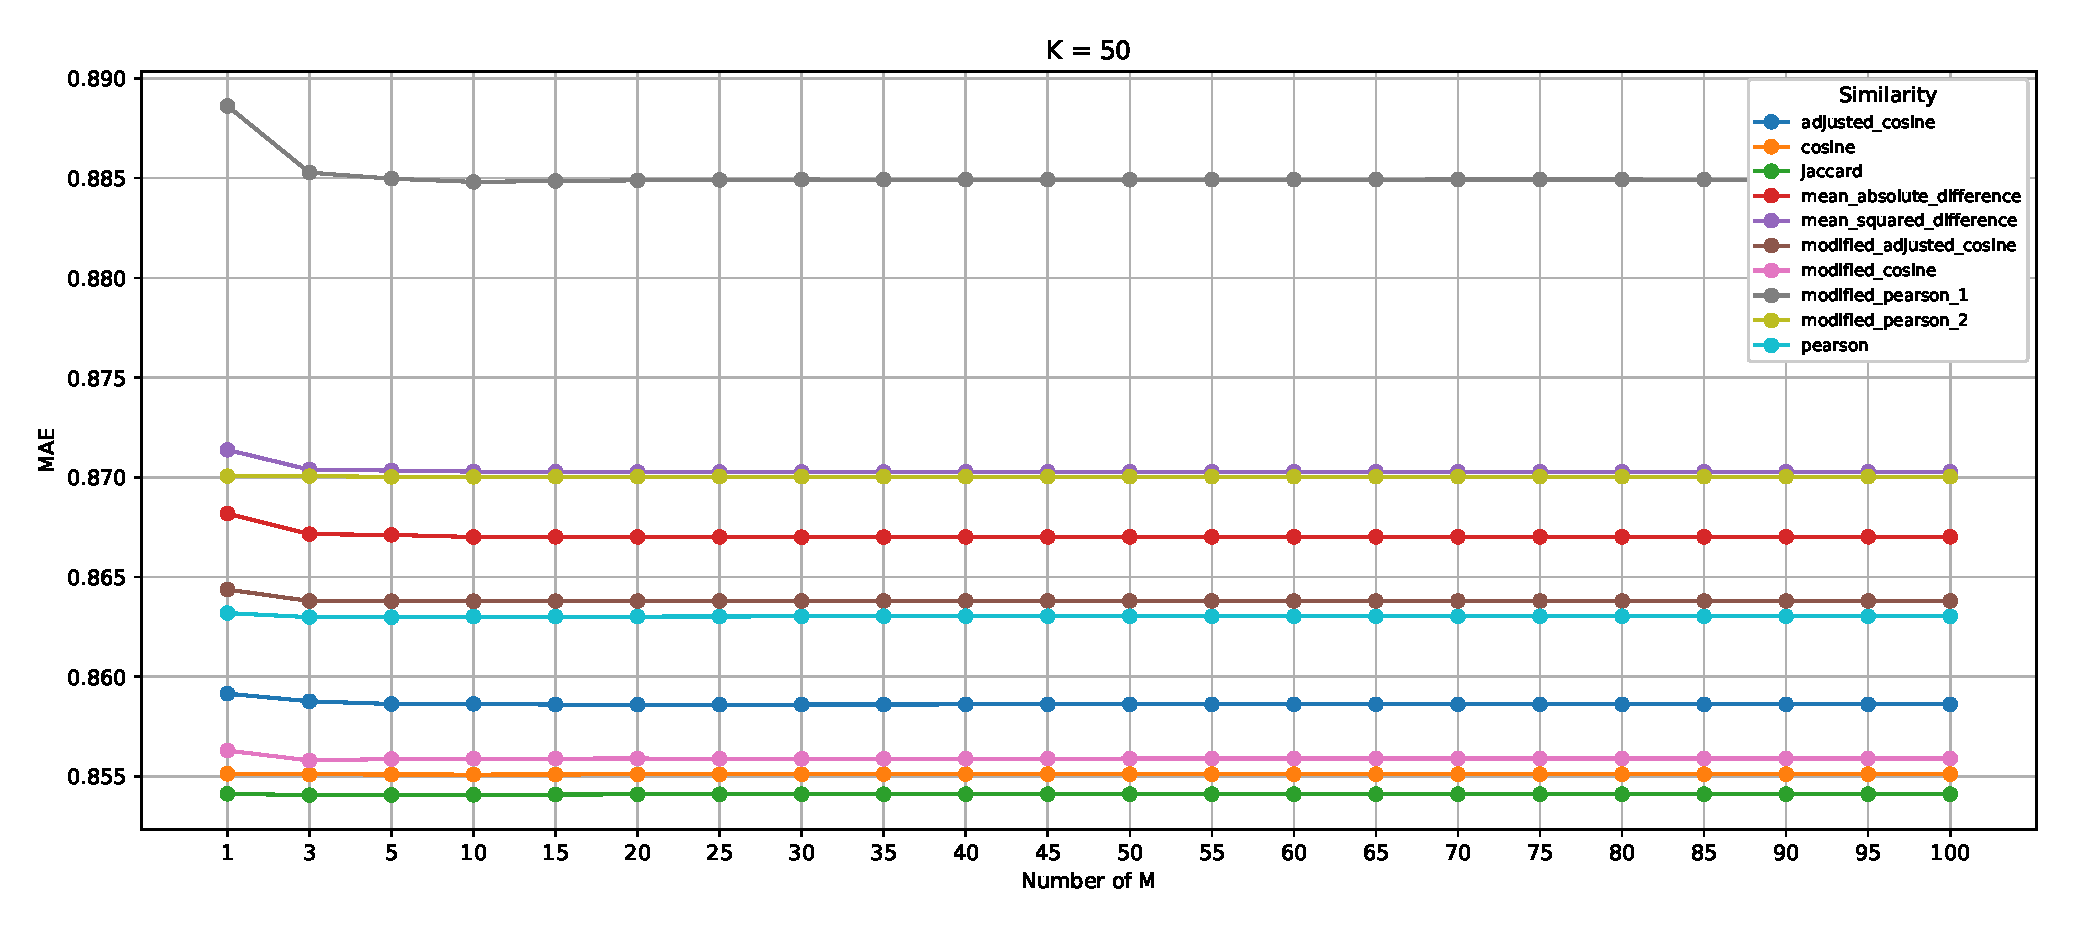
\includegraphics[width=1\textwidth,height=0.6\textheight]{evaluation_user_mae.eps}
        \end{figure}
        \centering
        \tiny
        Jaccard coefficient at K=50 \& M=3, MAE=0.854066176
    \end{columns}
\end{frame}
\begin{frame}[t]
    \frametitle{User-based KNN and Recursive-KNN RMSUE}
    \vspace{-0.7cm}
    \begin{columns}
        \column{0.5\textwidth}
        \centering
        \underline{\textbf{KNN}}
    \begin{figure}
    \centering
    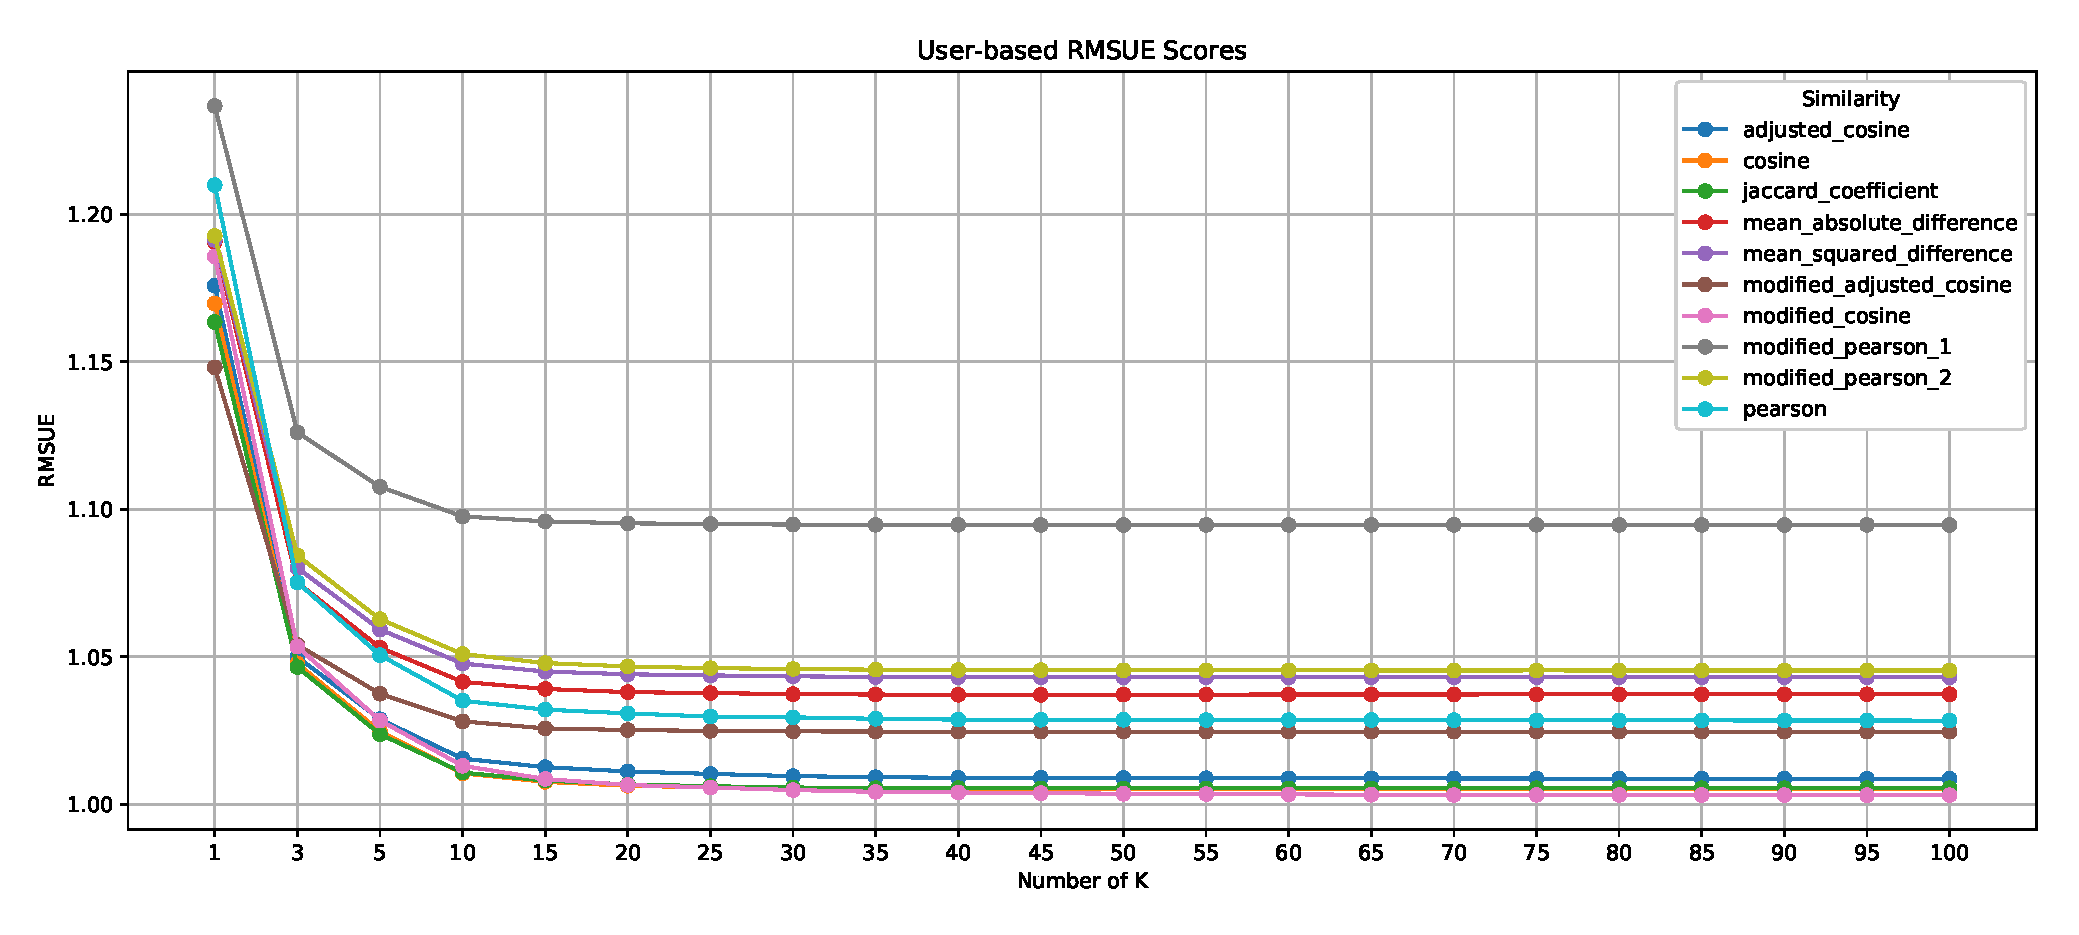
\includegraphics[width=1\textwidth,height=0.6\textheight]{User_RMSUE_KNN.eps}
    \end{figure}
    \centering
    \tiny
    Modified cosine at K=100, RMSUE=1.0031145695
        \column{0.5\textwidth}
        \centering
        \underline{\textbf{Recursive-KNN}}
    \begin{figure}
    \centering
    \includegraphics[width=1\textwidth,height=0.6\textheight]{evaluation_user_rmsue.eps}
    \end{figure}
    \centering
    \tiny
    Modified cosine at K=100 \& M=3, RMSUE=0.9089525549
\end{columns}
\end{frame}
\begin{frame}[t]
    \frametitle{User-based KNN and Recursive-KNN MAUE}
    \vspace{-0.7cm}
    \begin{columns}
        \column{0.5\textwidth}
        \centering
        \underline{\textbf{KNN}}
    \begin{figure}
    \centering
    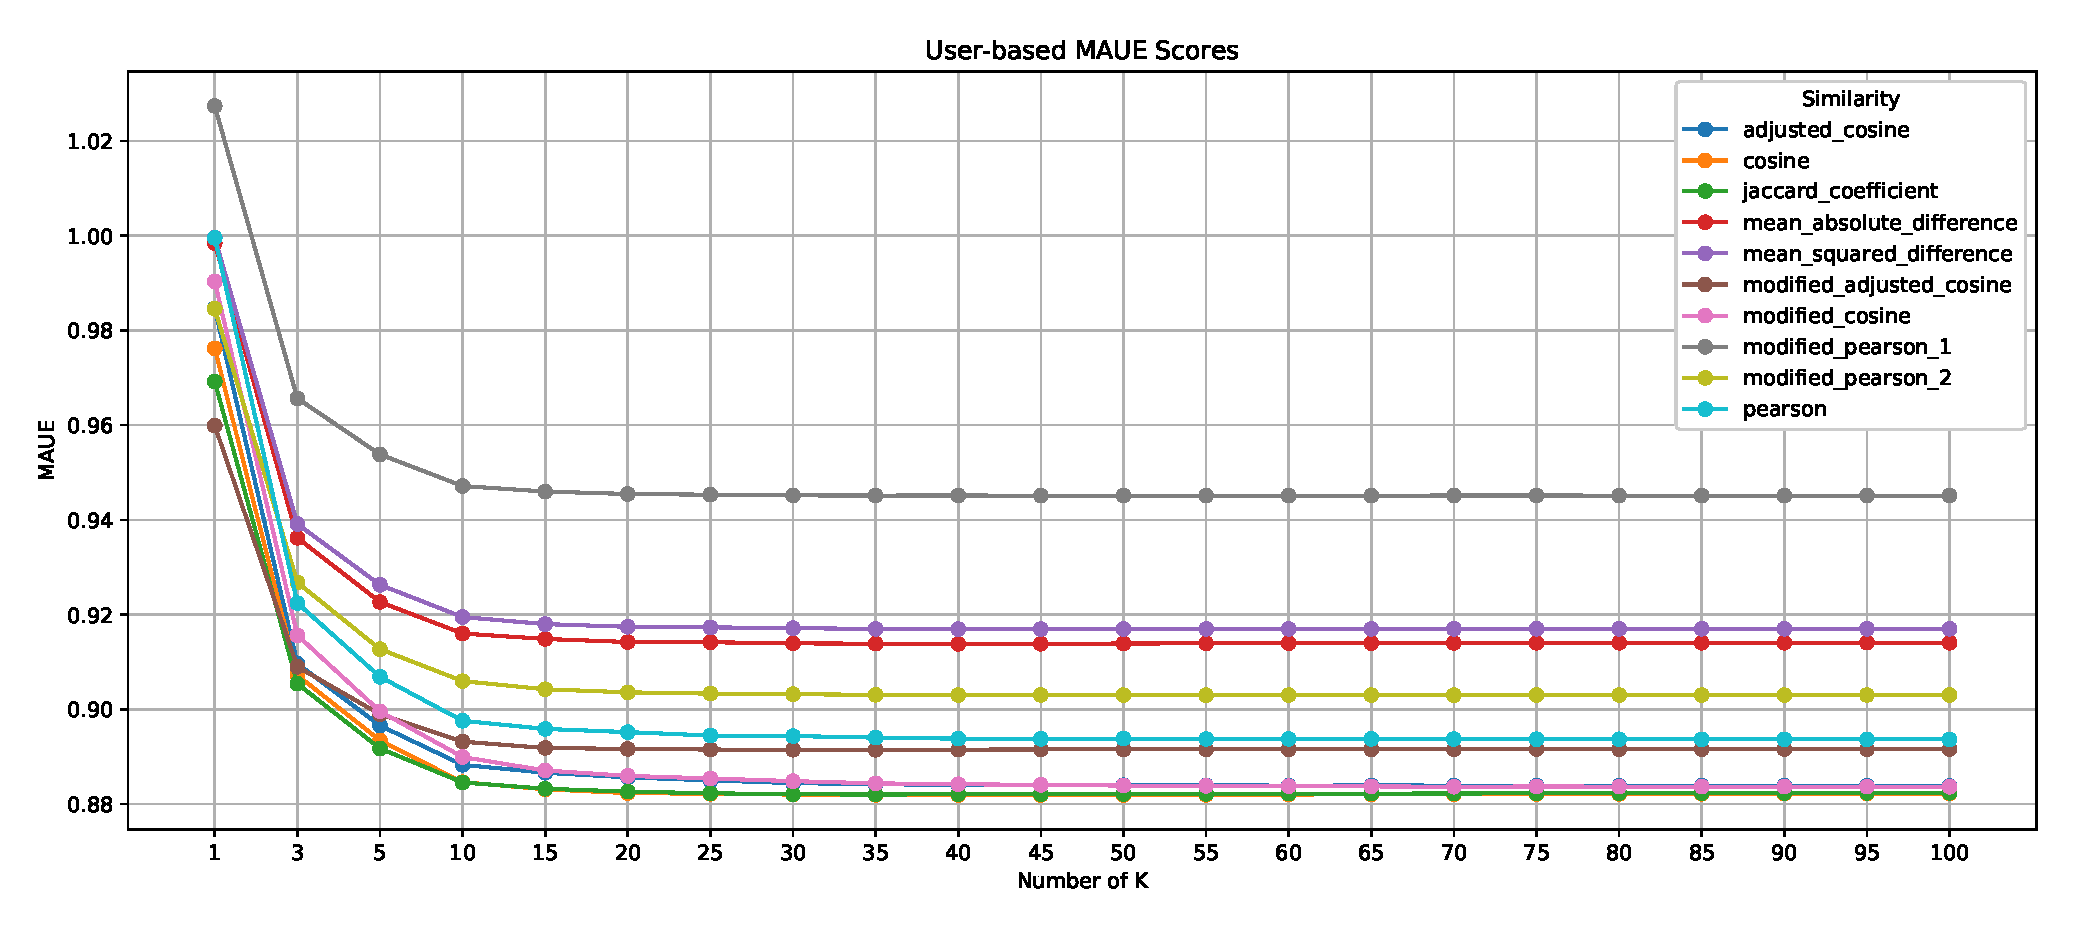
\includegraphics[width=1\textwidth,height=0.6\textheight]{User_MAUE_KNN.eps}
    \end{figure}
    \centering
    \tiny
    Cosine similarity at K=50, MAUE=0.8819077974
        \column{0.5\textwidth}
        \centering
        \underline{\textbf{Recursive-KNN}}
    \begin{figure}
    \centering
    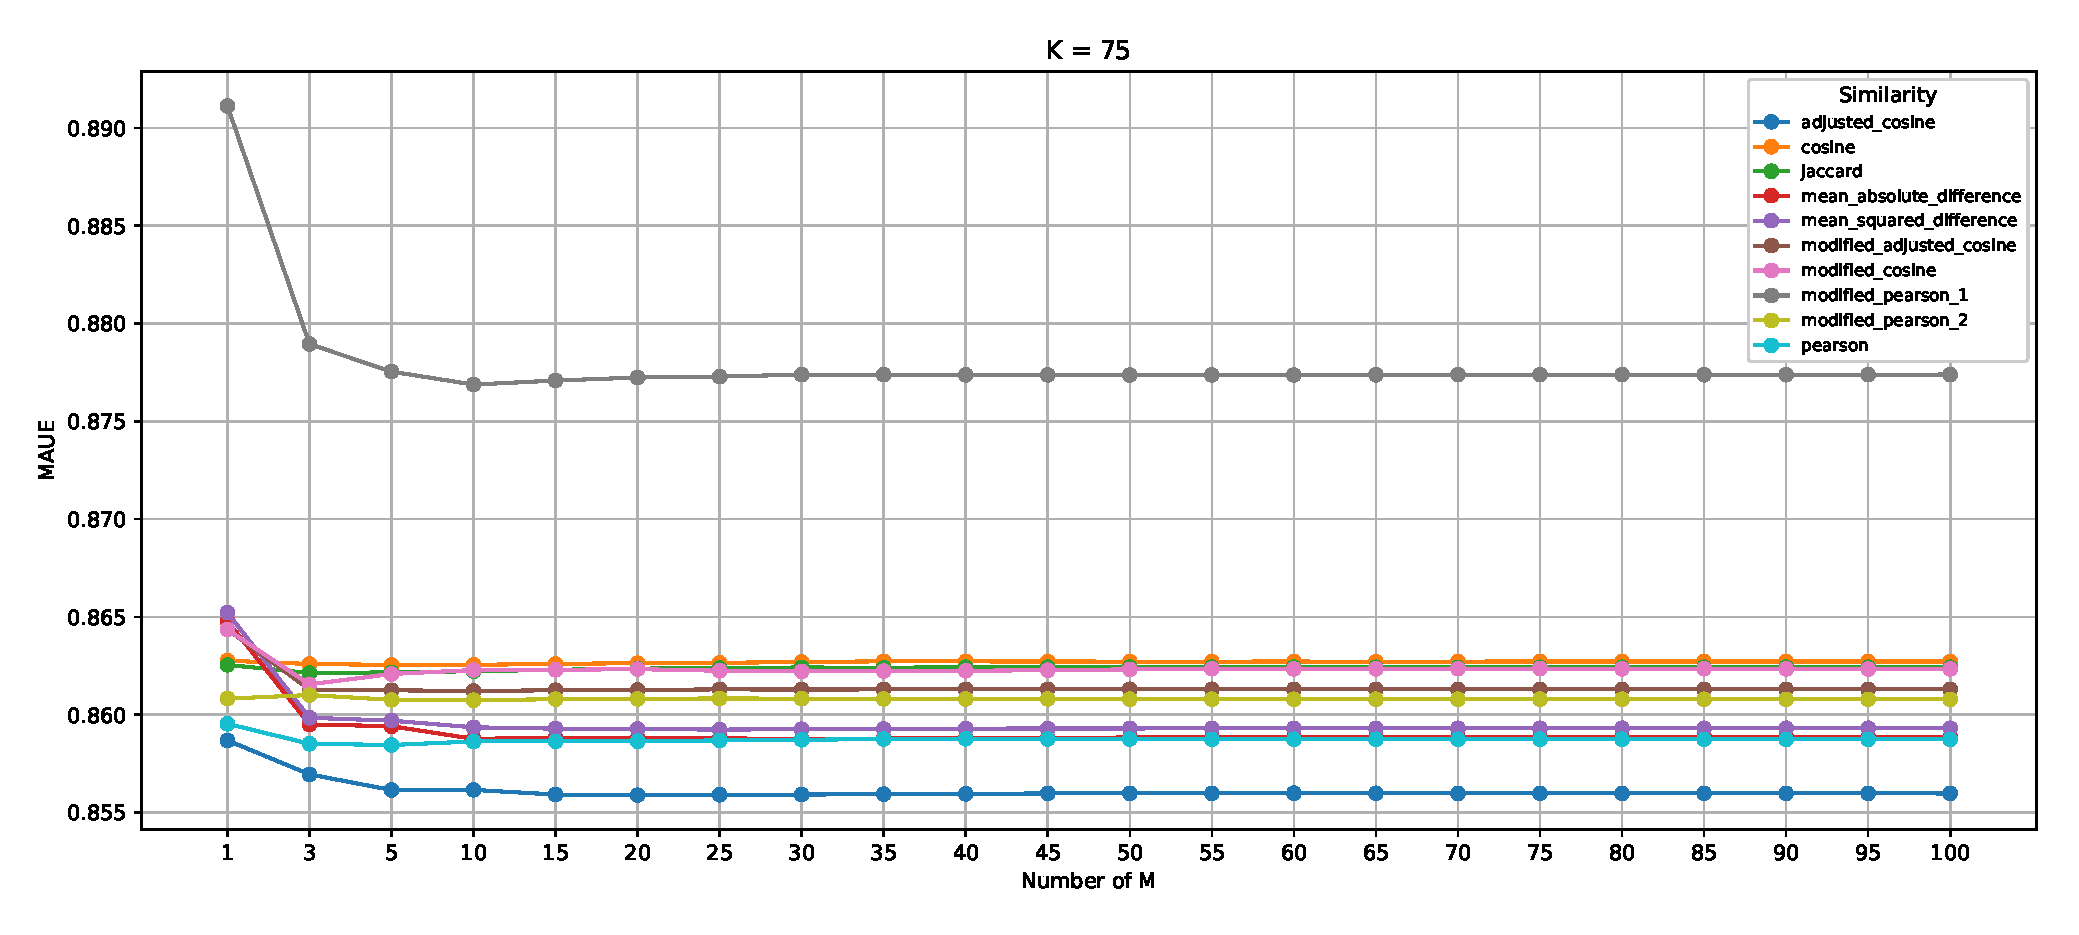
\includegraphics[width=1\textwidth,height=0.6\textheight]{evaluation_user_maue.eps}
    \end{figure}
    \centering
    \tiny
    Adjusted cosine at K=75 \& M=20, MAUE=0.8558869566
\end{columns}
\end{frame}
\begin{frame}[t]
    \frametitle{Item-based KNN and Total RMSE}
    \vspace{-0.7cm}
    \begin{columns}
        \column{0.5\textwidth}
        \centering
        \underline{\textbf{KNN}}
    \begin{figure}
    \centering
    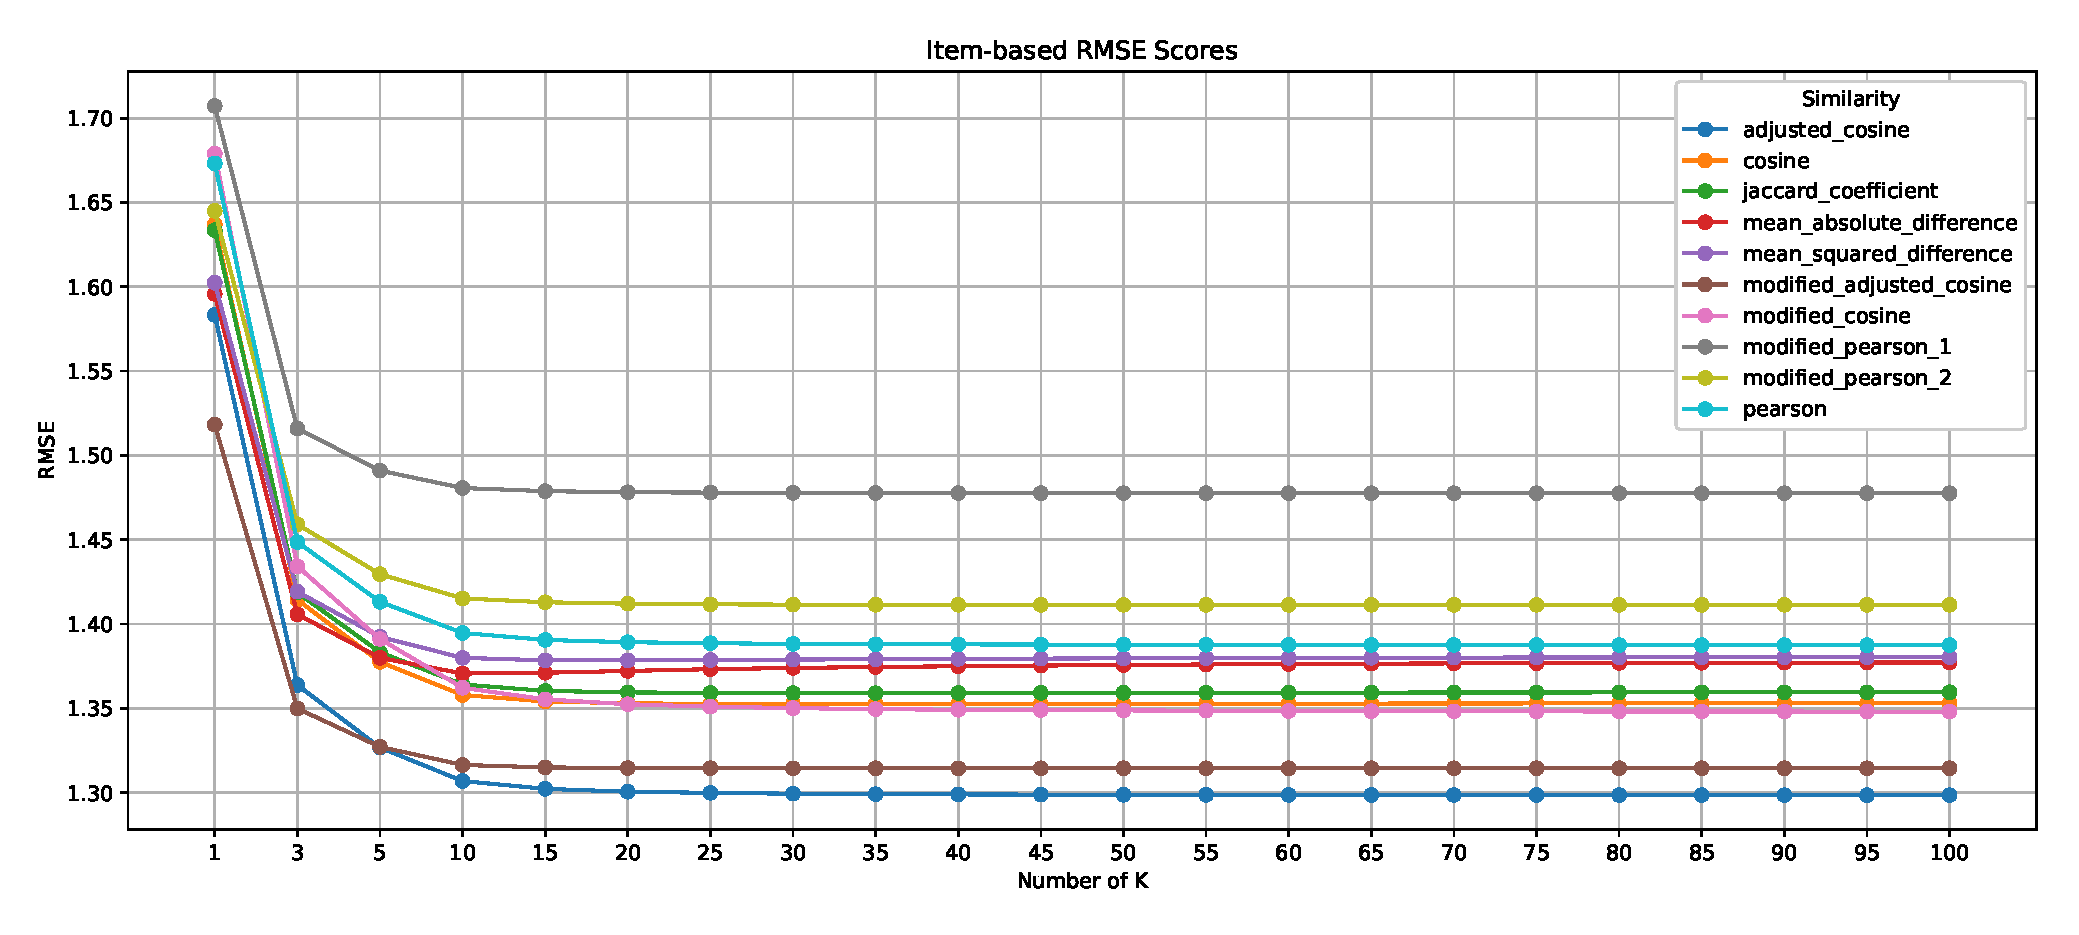
\includegraphics[width=1\textwidth,height=0.6\textheight]{Item_RMSE_KNN.eps}
    \end{figure}
    \centering
    \tiny
    Adjusted cosine at K=95, RMSE=1.2984970982
        \column{0.5\textwidth}
        \centering
        \underline{\textbf{Total}}
    \begin{figure}
    \centering
    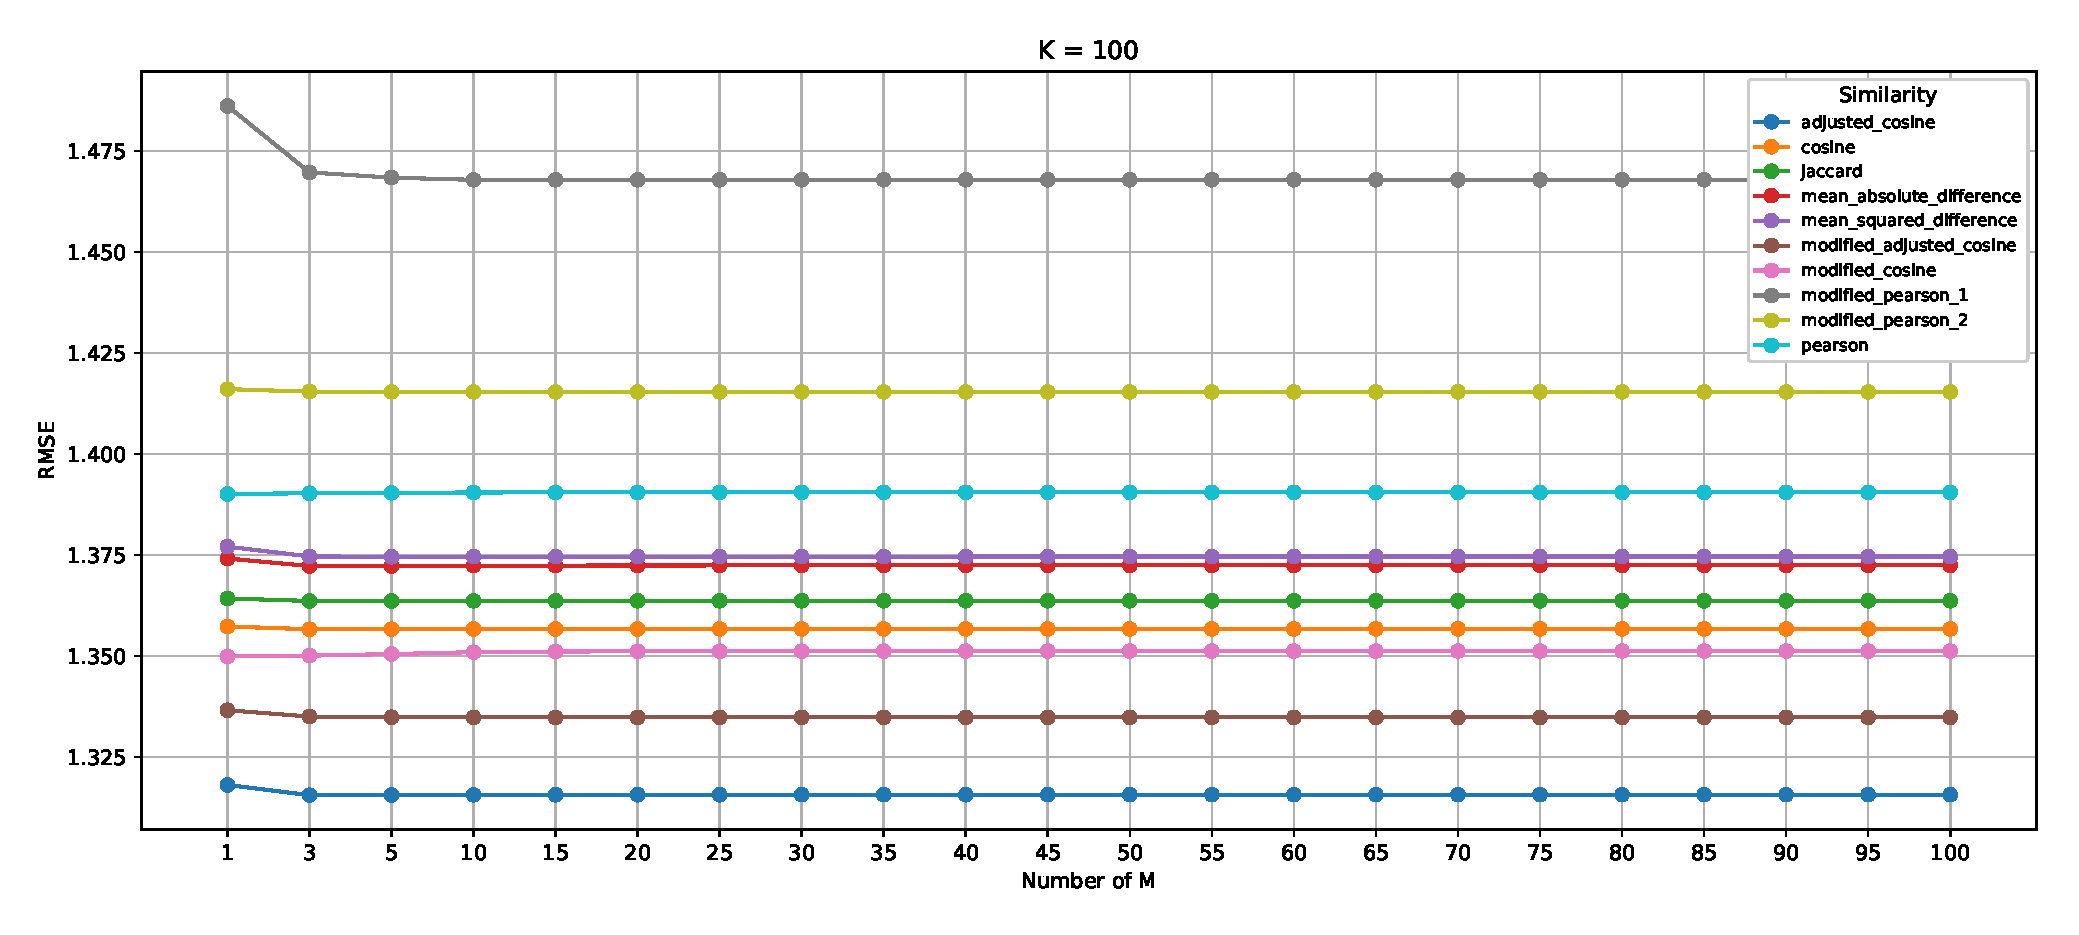
\includegraphics[width=1\textwidth,height=0.6\textheight]{evaluation_item_rmse.eps}
    \end{figure}
    \centering
    \tiny
    Adjusted cosine at K=100 \& M=3, RMSE=1.3155259043
\end{columns}
\end{frame}
\begin{frame}[t]
    \frametitle{Item-based KNN and Total MAE}
        \vspace{-0.7cm}
        \begin{columns}
            \column{0.5\textwidth}
            \centering
            \underline{\textbf{KNN}}
        \begin{figure}
        \centering
        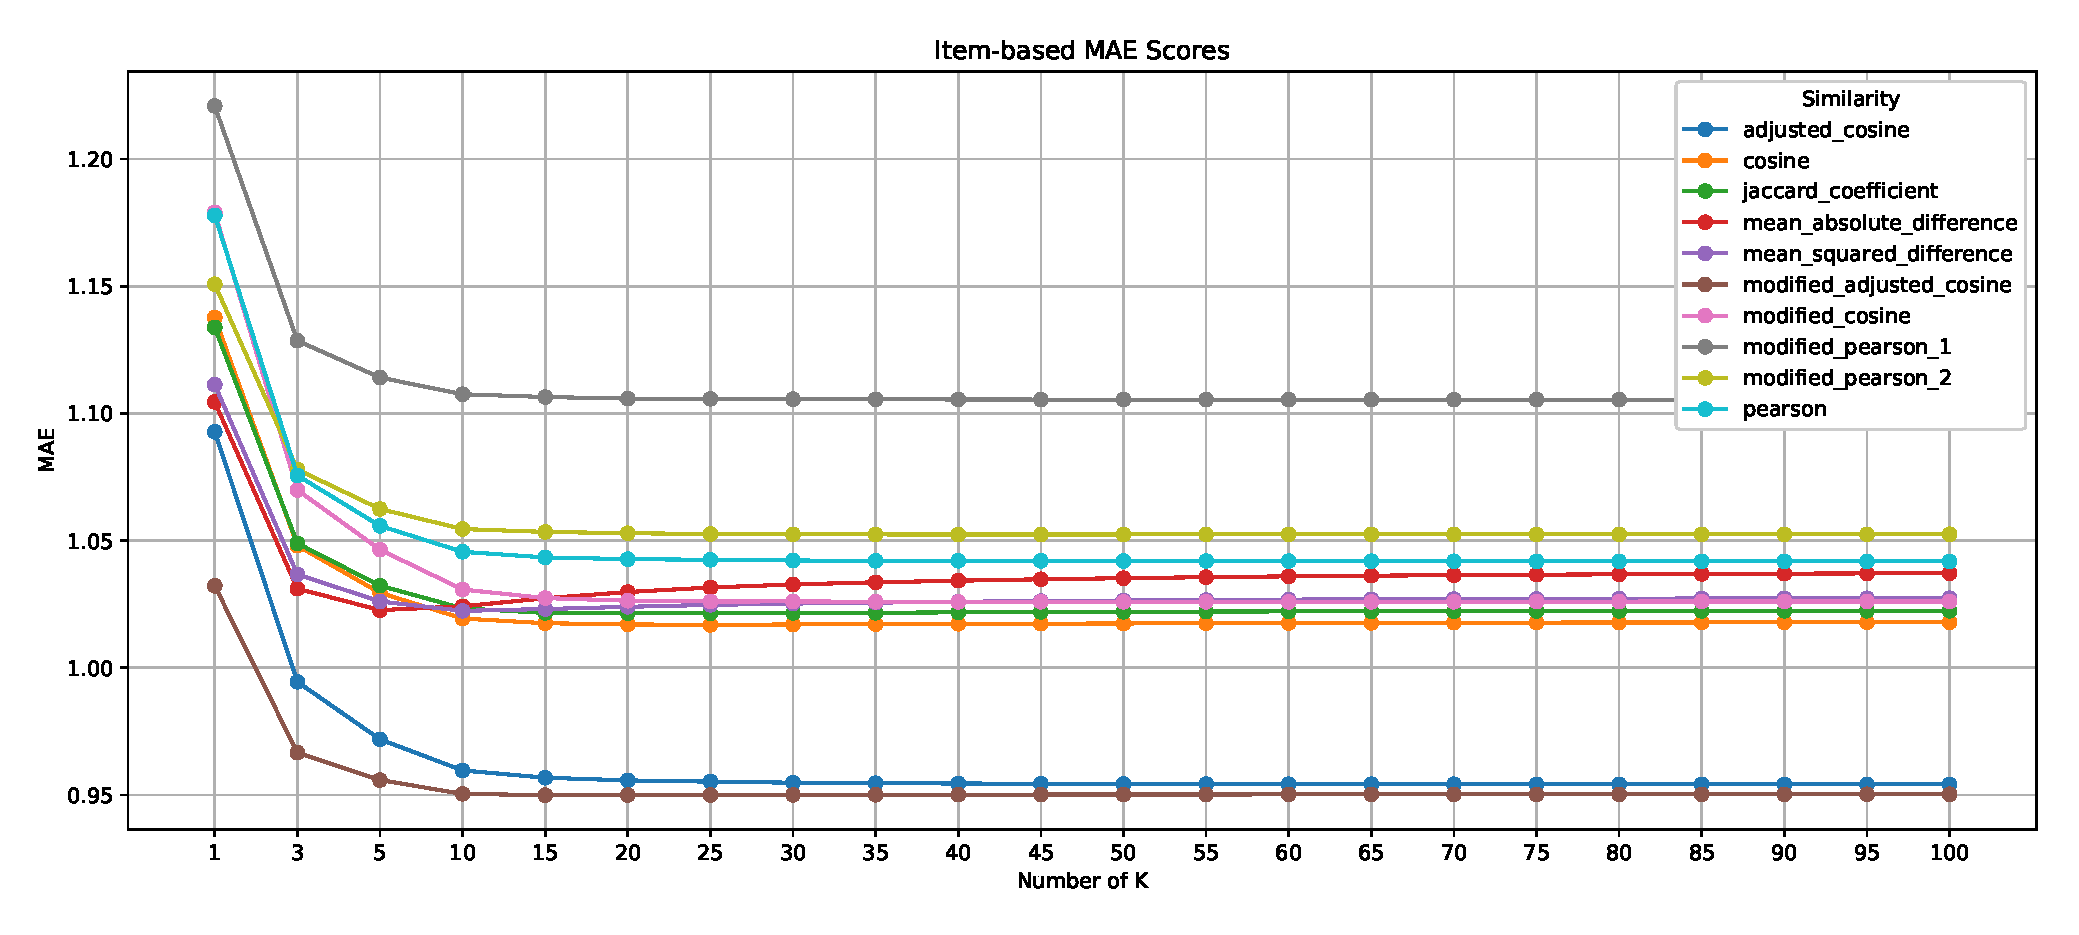
\includegraphics[width=1\textwidth,height=0.6\textheight]{Item_MAE_KNN.eps}
        \end{figure}
        \centering
        \tiny
        Modified adjusted cosine at K=15, MAE=0.9499219326
            \column{0.5\textwidth}
            \centering
            \underline{\textbf{Total}}
        \begin{figure}
        \centering
        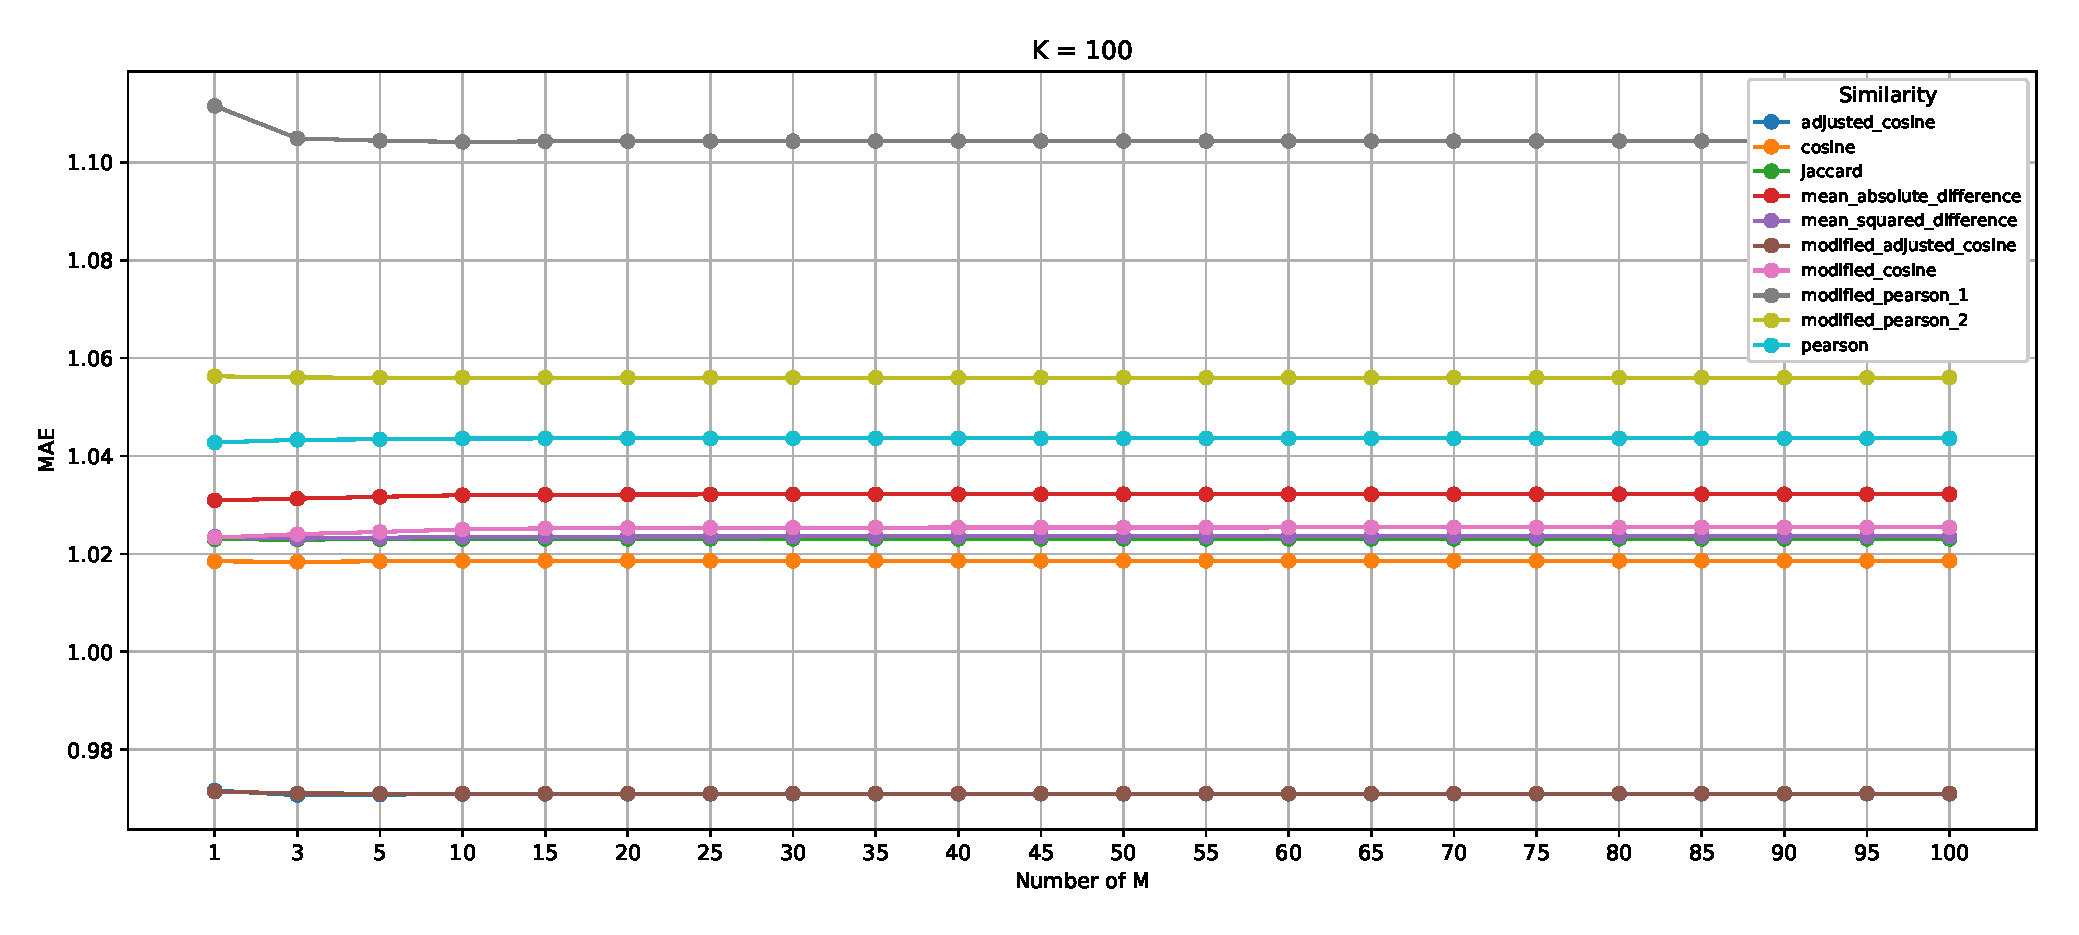
\includegraphics[width=1\textwidth,height=0.6\textheight]{evaluation_item_mae.eps}
        \end{figure}
        \centering
        \tiny
        Adjusted cosine at K=100 \& M=3, MAE=0.9707211649
    \end{columns}
\end{frame}
\begin{frame}[t]
    \frametitle{Item-based KNN and Recursive-KNN RMSUE}
    \vspace{-0.7cm}
    \begin{columns}
        \column{0.5\textwidth}
        \centering
        \underline{\textbf{KNN}}
    \begin{figure}
    \centering
    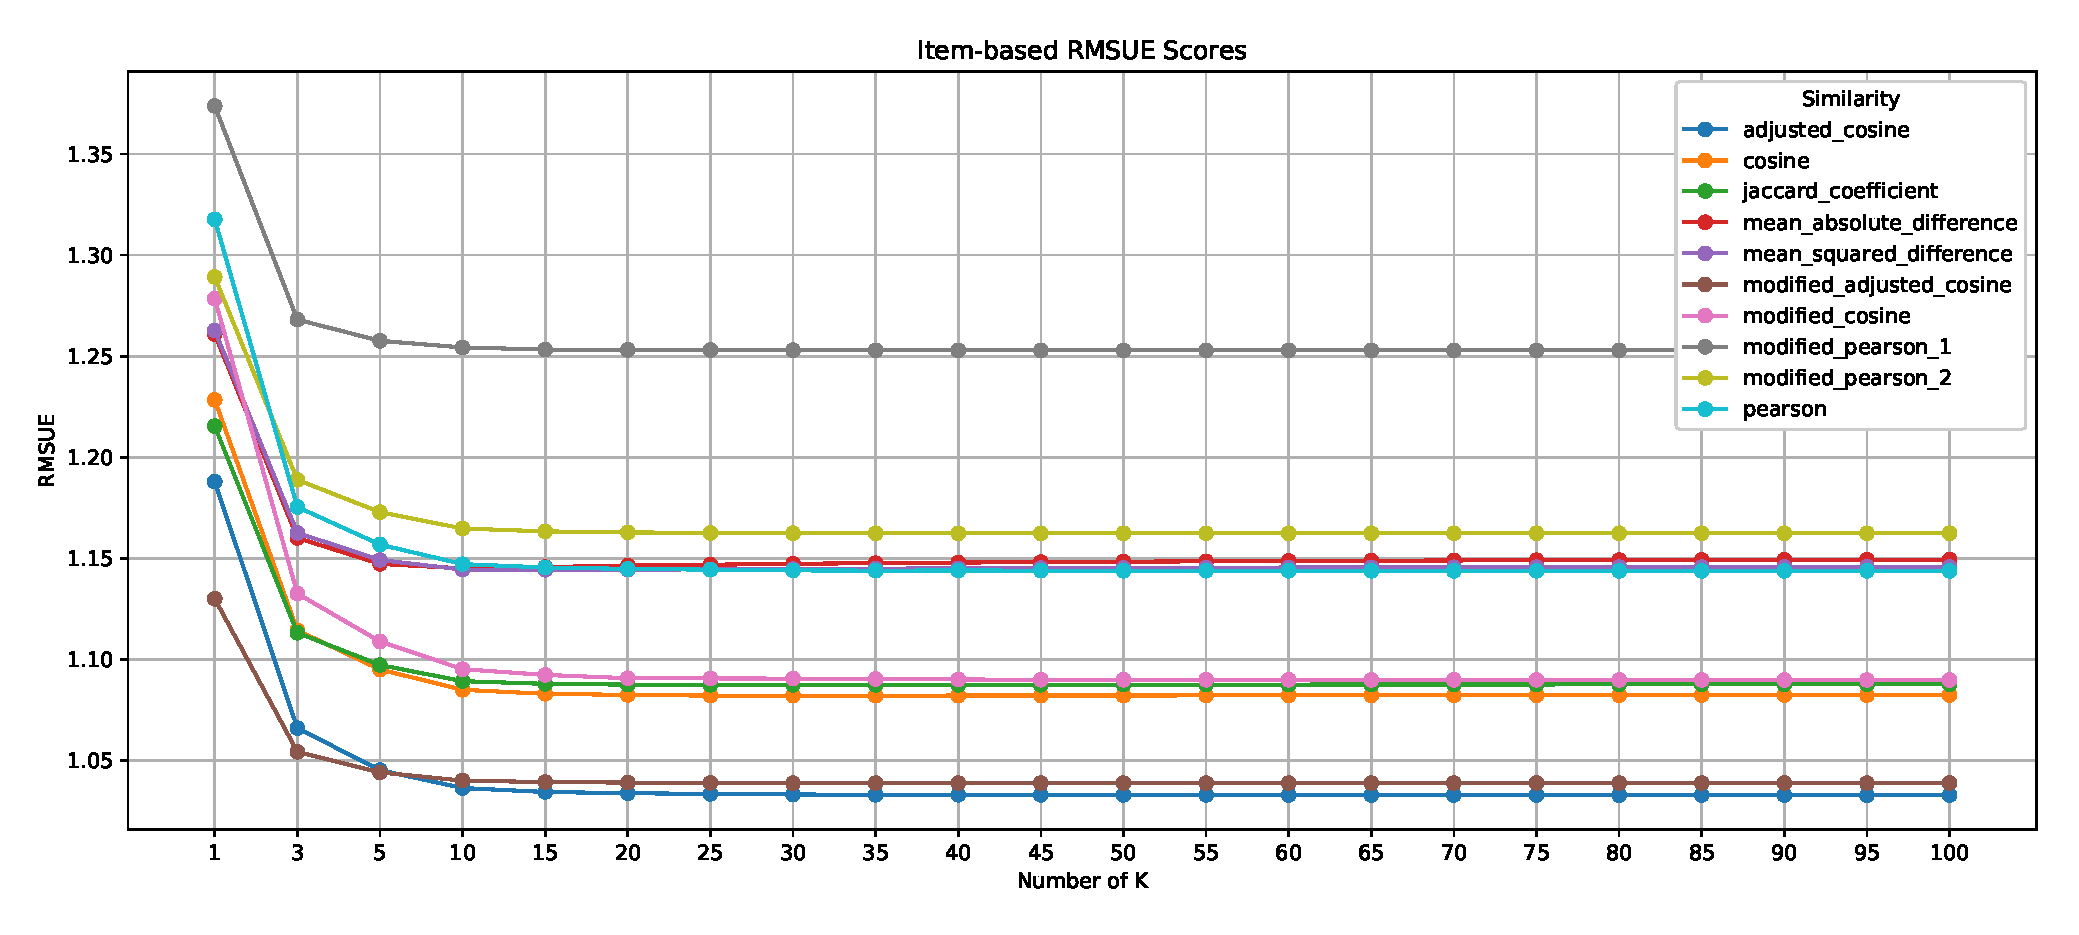
\includegraphics[width=1\textwidth,height=0.6\textheight]{Item_RMSUE_KNN.eps}
    \end{figure}
    \centering
    \tiny
    Adjusted cosine at K=100, RMSUE=1.0328968801
        \column{0.5\textwidth}
        \centering
        \underline{\textbf{Recursive-KNN}}
    \begin{figure}
    \centering
    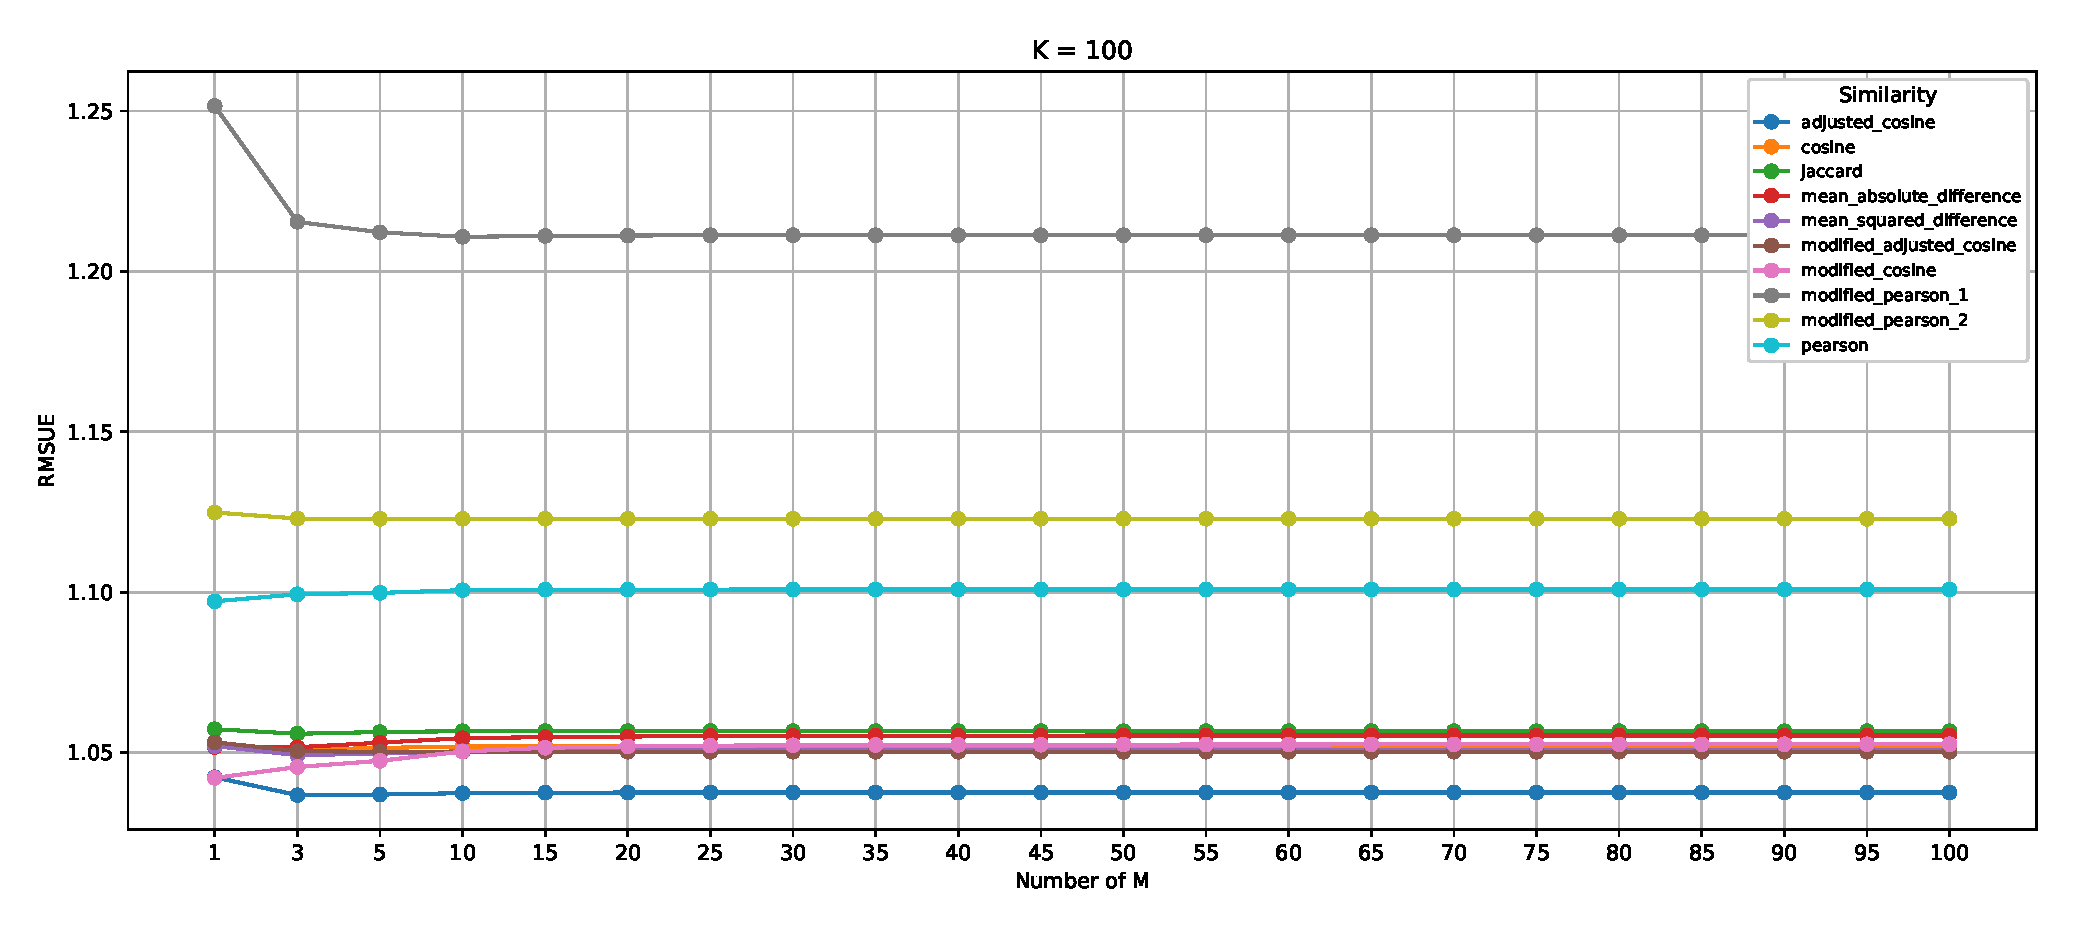
\includegraphics[width=1\textwidth,height=0.6\textheight]{evaluation_item_rmsue.eps}
    \end{figure}
    \centering
    \tiny
    Adjusted cosine at K=100 \& M=3, RMSUE=1.0367245756
\end{columns}
\end{frame}
\begin{frame}[t]
    \frametitle{Item-based KNN and Recursive-KNN MAUE}
    \vspace{-0.7cm}
    \begin{columns}
        \column{0.5\textwidth}
        \centering
        \underline{\textbf{KNN}}
    \begin{figure}
    \centering
    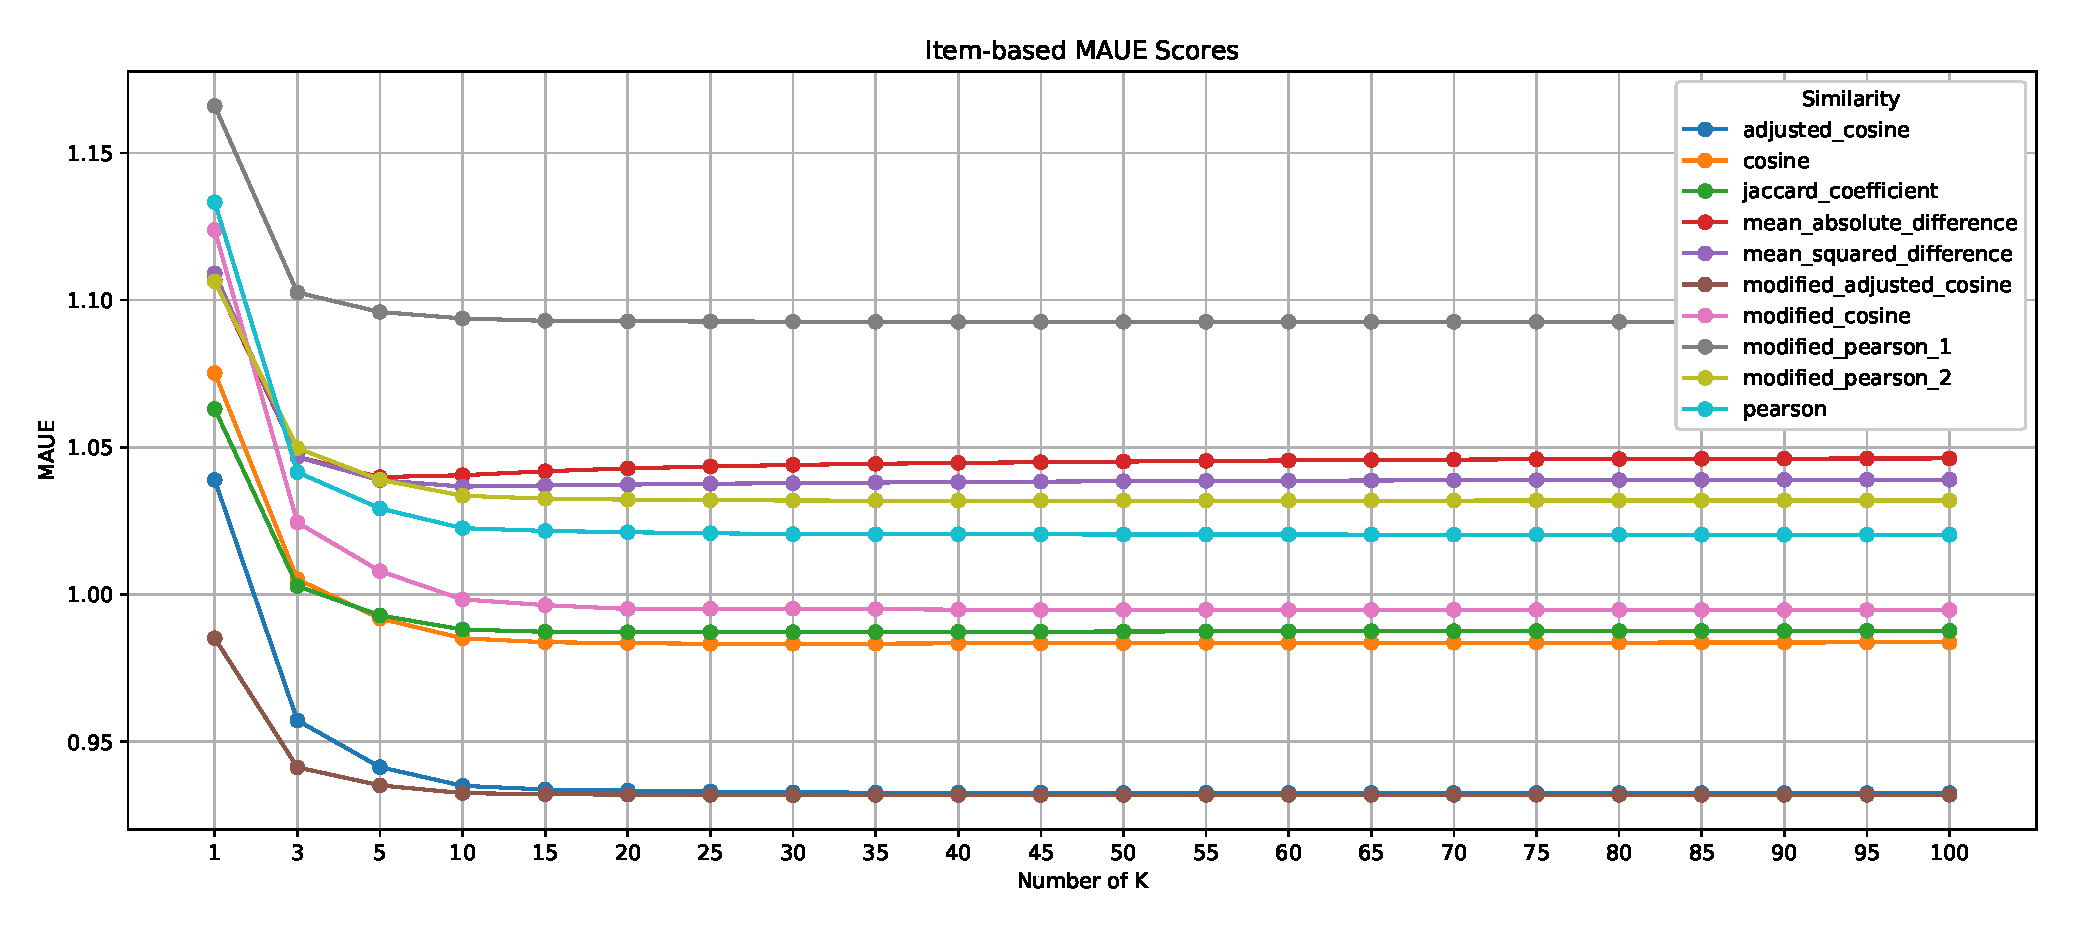
\includegraphics[width=1\textwidth,height=0.6\textheight]{Item_MAUE_KNN.eps}
    \end{figure}
    \centering
    \tiny
    Modified adjusted cosine at K=30, MAUE=0.9318609947
        \column{0.5\textwidth}
        \centering
        \underline{\textbf{Recursive-KNN}}
    \begin{figure}
    \centering
    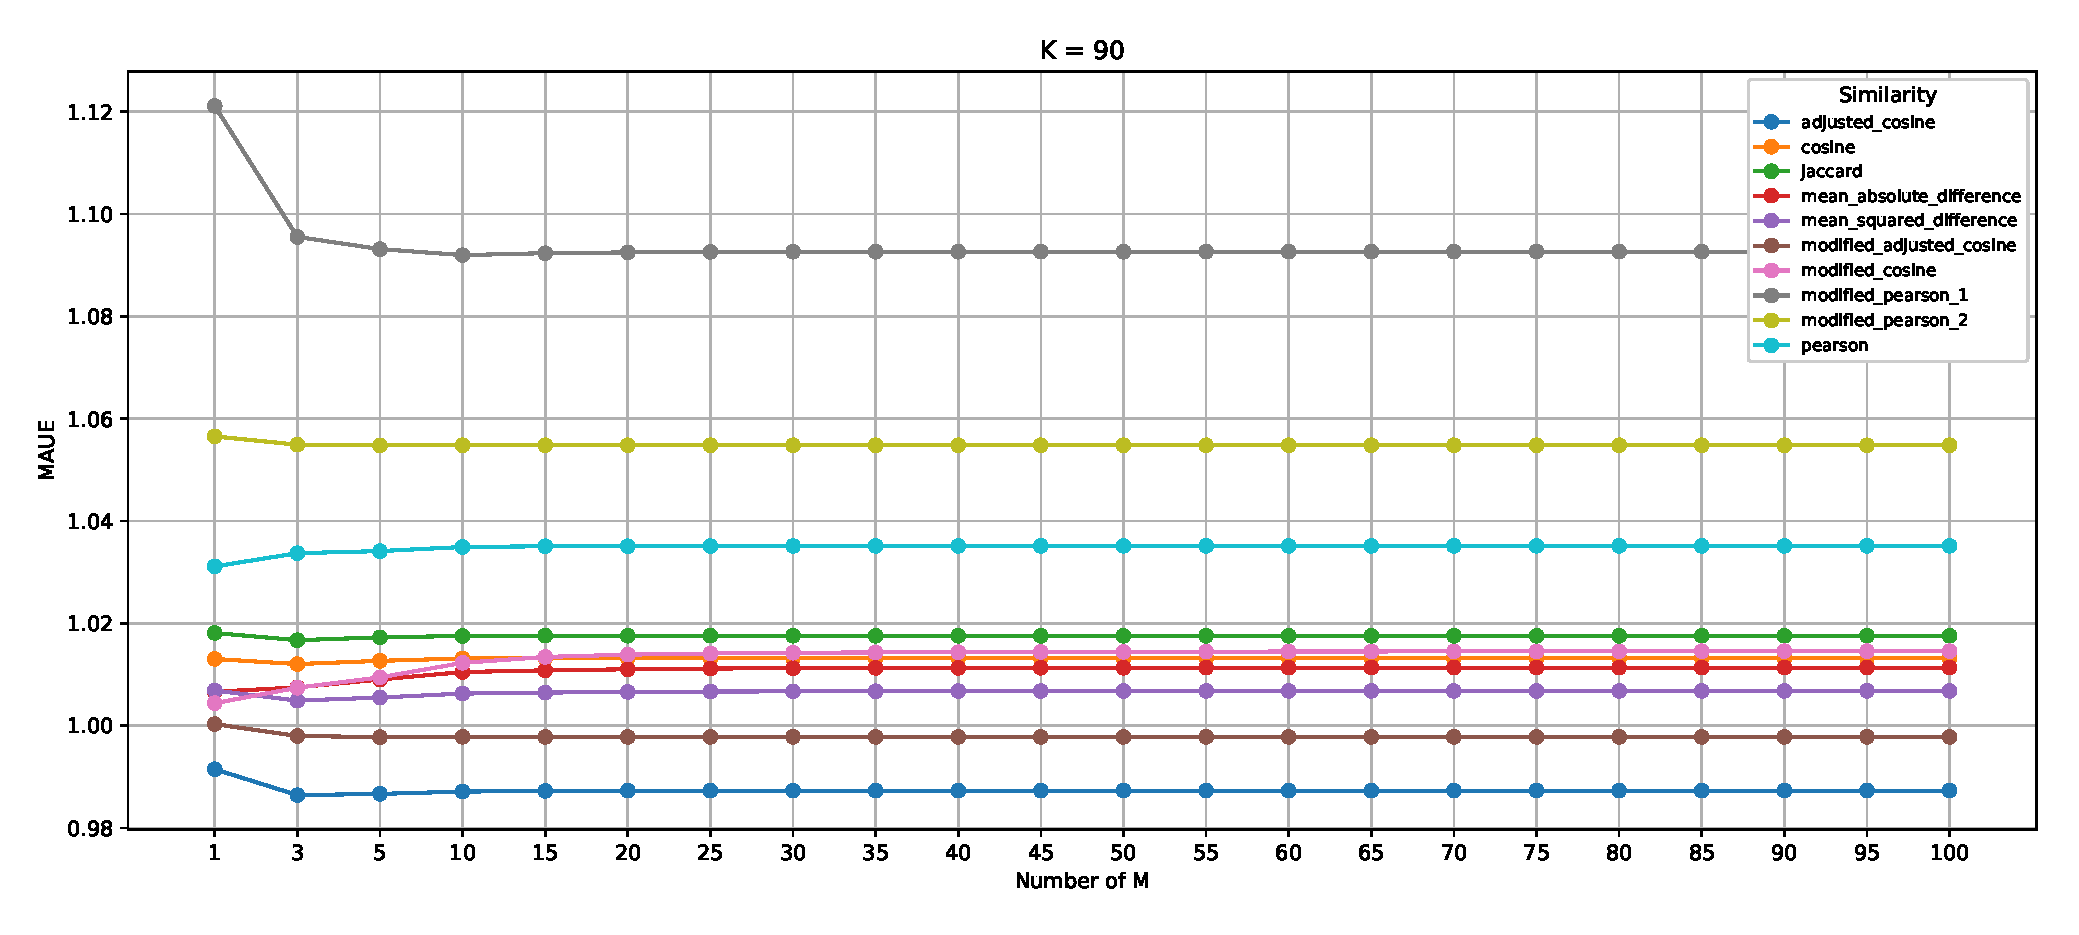
\includegraphics[width=1\textwidth,height=0.6\textheight]{evaluation_item_maue.eps}
    \end{figure}
    \centering
    \tiny
    Adjusted cosine at K=90 \& M=3, MAUE=0.9864005988
\end{columns}
\end{frame}
